\section{Analysis Parameters}
\subsection{Attenuation Relationship}

The choice of the ground motion attenuation relationship, as a highly influential factor, is of a great importance in seismic hazard analysis. \citet{Zafarani2014} used 163 free-field acceleration time histories recorded at epicentral distance of up to 200 km from 32 earthquakes to investigate the predictive capabilities of the local, regional, and next generation attenuation (NGA) ground-motion prediction equations and determined their applicability for northern Iran. After evaluating different Ground Motion Prediction Equations, \citet{Kalkan2004}, \citet{Chiou2008}, and \citet{Boore2008} represented suitable performance for  PGA  with LLH (Log-Likelihood method) score of 1.54, 1.55, and 1.59. Mean of the mentioned attenuation relationships (not shown here), are very close together, especially at higher magnitude. Using \citet{Scherbaum2009} approach and \citet{Zafarani2014} coefficients we calculated the logic tree weights as 0.3376, 0.3354, and 0.3270, respectively. The epistemic uncertainty in attenuation relationship is being considered through using the logic tree approach. Having close mean value and similar logic tree weights, logic tree approach will have a minor effect in considering the epistemic uncertainty. In this study instead of using  different GMPEs we use the best model of attenuation relationship for PGA \citep{Zafarani2014} as well $\pm$ standard deviation. \\

\noindent
The attenuation relationship is:

\begin{equation}
\begin{split}
ln\ (Y) = b_1 + b_2(M_w-6) + b_3( M_w-6)^{2}+  \\ 
b_5ln\ r + b_V \ ln(V_S/V_A) \  with \  r= \sqrt{R{r^2_{cl} + h^2}}  
\end{split}
\end{equation}

\subsection{b-value}

For each of the three seismic regions, Gutenberg-Richter parameters and maximum magnitude ($M_{max}$) were calculated using Seismic Hazard Assessment code (HA3) \citep{kijko2004}. The regional maximum magnitude for each region is estimated by the \citet{Kijko1989} method, which is implemented in the HA3 package. For smoothed seismicity areas, $b-value$ is assumed constant. The $a-value$ can vary spatially and is determined by counting earthquakes above $M$ 3.0 in each grid cells.\\
\noindent
\citet{Karimiparidari2013} applied the Maximum Curvature (MAXC) technique \citep{Wyss1999, Wiemer2000} by ZMap \citep{Wiemer2001} to calculate the level of completeness of instrumental part of the catalog.  Following the \citet{Karimiparidari2013}, we assume the catalog is complete for earthquakes with magnitude 4.5, 4.4, 4.5, 4.5, and 4.4 for Azerbaijan, Alborz,  Kopeh-Dagh, Central Iran, and Zagros tectonic seismic regions, respectively. For the uniform model we used 4.5 as a completeness magnitude. In this study we use those magnitudes of completeness as the magnitude threshold in the calculation of the seismicity parameters. We also used the seismicity parameters of \citet{Karimiparidari2013} as the priory information in HA3 code. The updated values are displayed in Table \ref{tab:b_value}.  Annual occurrence rate of the earthquake for each region is shown in Fig.~\ref{fig:annual_m}.

\begin{figure*} [!ht]
\centering
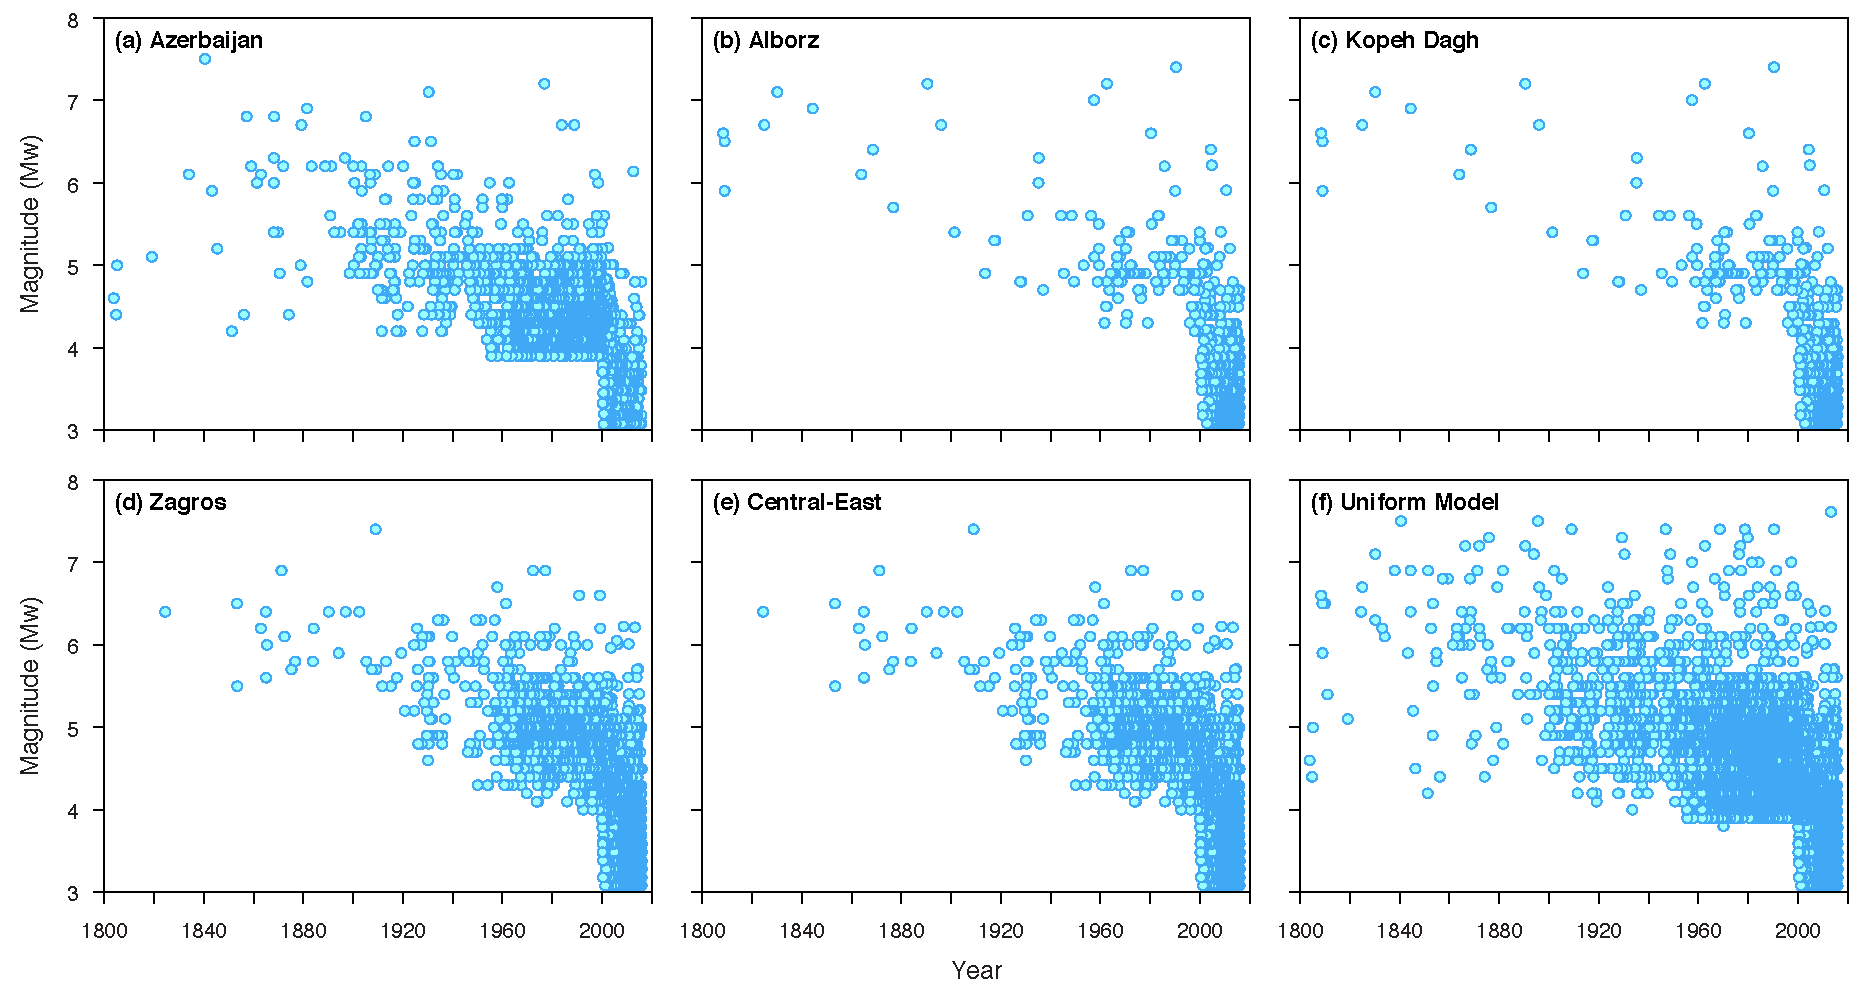
\includegraphics[scale=0.3]{figures/pdf/figure-04} 
\caption{The annual probability of exceeding the specified magnitude in different seismic tectonic region (a) Alborz, b) Azerbaijan, c) Central, d) Kopeh Dagh, e) Uniform f) Zagros). The margin display the positive and negative standard deviation.}
\label{fig:annual_m}
\end{figure*}


\noindent


\begin{table*}[!ht]
\centering
\caption{Seismicity parameters for three tectonic seismic regions.}
    \begin{tabular}{ccccc}
    ~                          &         $b-value$     &   $M_{max} $  Calculated & $M_{max}$ obseved \\ \hline
    Azerbaijan           & 1.1   $\pm$ 0.03   &   7.93  $\pm$  0.34           &   7.7      			    \\ \hline
    Alborz                  &1.03  $\pm$ 0.03   &   7.85  $\pm$  0.66           &   7.8          	            \\ \hline
    Kopeh Dagh        & 0.89 $\pm$ 0.04   &   7.78  $\pm$  0.31           &   7.6          	            \\ \hline
    Central Iran         & 0.95 $\pm$ 0.04   &   7.84  $\pm$  0.34           &   7.6                           \\ \hline
    Zagros                 & 0.99 $\pm$ 0.02  &   7.47  $\pm$  0.26            &  7.4                            \\ \hline
    Uniform Model    & 0.9    $\pm$ 0.02  &   7.87  $\pm$  0.26            &  7.8                            \\ 
    \end{tabular}
 \label{tab:b_value} 
\end{table*}

\subsection{Catalog Completness}
For the smoothed seismicity method, completeness of each magnitude in the catalog is an important factor.  \citet{Frankel1995} plotted the cumulative number of events against time for different regions. He assumes that from the point that the line become linear, the catalog is complete. This approach is similar to the MAXC method of ZMAP software \citep{Wiemer2001}, where the completeness treshold is the maximum value of the first derivative of the frequency-magnitude curve. Using the cumulative frequency-magnitude distribution of \citet{Gutenberg1944} and also frequency magnitude distribution approach in software ZMAP, \citet{Zare2014} reported the catalog completeness for the study regions. World widely large earthquakes were routinely located after increasing number of seismic stations establishment in the early 1900s \citep{Shearer2009}. Up to 1961 these data formed the early instrumental period. In 1961 the Worldwide Standardized Seismograph Network (WWSSN) was stablished. The record of these seismographs considerably improved the seismic catalogs in different part of the world \citep{Shearer2009}. Fig.~\ref{fig:completness_scatter} shows the magnitude distribution of events with respect to the time of occurrence of the events.

\begin{figure*} [!ht]
\centering
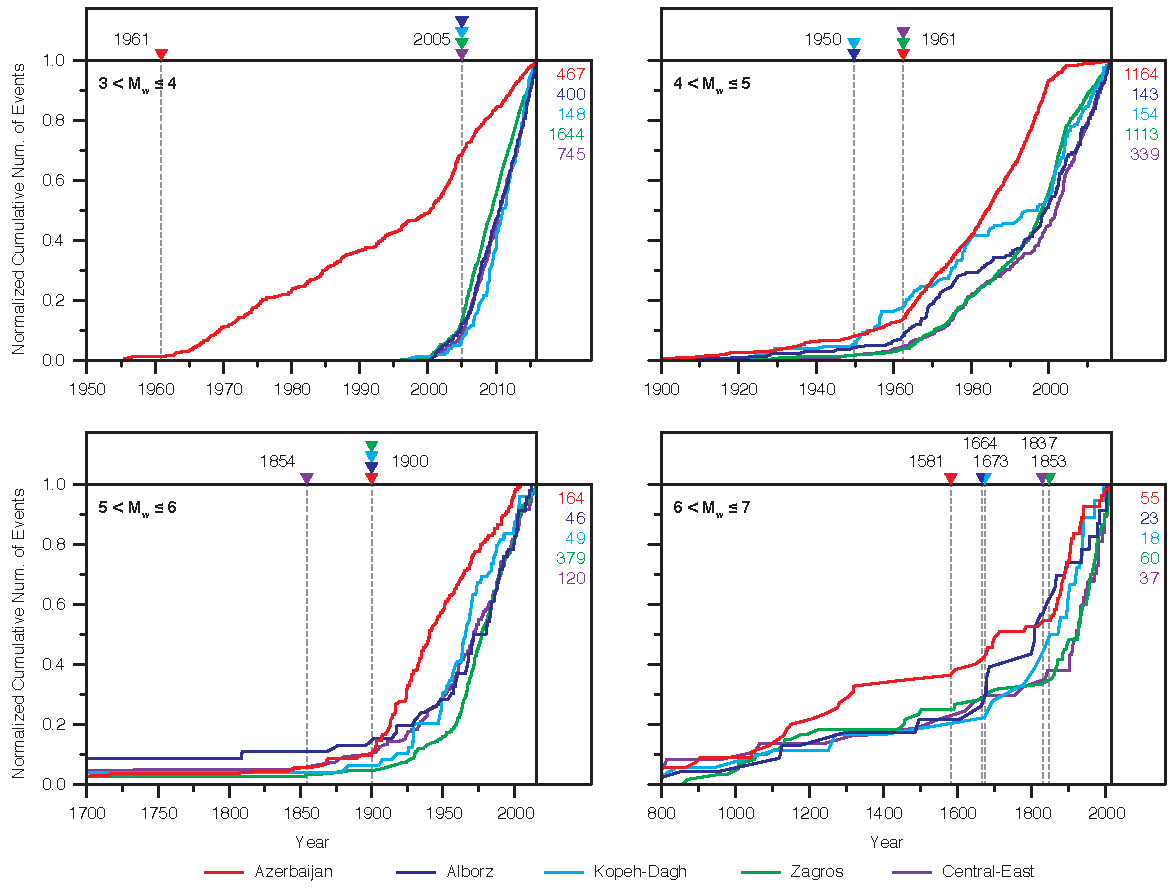
\includegraphics[scale=0.5]{figures/pdf/figure-05.pdf} 
\caption{Magnitude-time distribution of earthquakes in the study regions. a) Alborz, b) Azerbaijan, c) Central, d) Kopeh Dagh, e) Uniform f) Zagros}
\label{fig:completness_scatter}
\end{figure*}

 According to   \citet{Frankel1995},  we made plots of the cumulative number of events against time for different regions' catalog. We pick the Mw 0.5 increments in magnitude to be able to compare the results with \citet{Zare2014}. In order to be able to compare the results with \citet{Zare2014} we merge the data of Azerbaijan and Alborz seismic regions.  Fig.~\ref{fig:completness_compare_zare_2014_Az_Al} shows the completeness of catalog for earthquakes with different magnitude range in Azerbaijan-Alborz region. According to this figure, midrange magnitudes ($ 4 < Mw < 6 $) fairly obey the network developments in 1900 and 1961. The completeness thresholds for each magnitude range which are reported by \citet{Zare2014} are shown by dashed green line. In this study we follow the \citet{Frankel1995} approach to determine the completeness of each region. Even though the approach used by \citet{Frankel1995} will lead to the conservative results, we make sure that we don't use a period of time without knowing the complete number of events. Determining the completeness of the catalog is very sensitive to the data. Converting earthquake magnitudes from different scales to moment magnitude obviously has some error. Having broader range of magnitude will help to minimize these sort of error. In this study we consider the magnitude intervals for completeness study as $Mw = 1$. 

\begin{figure*} [!ht]
\centering
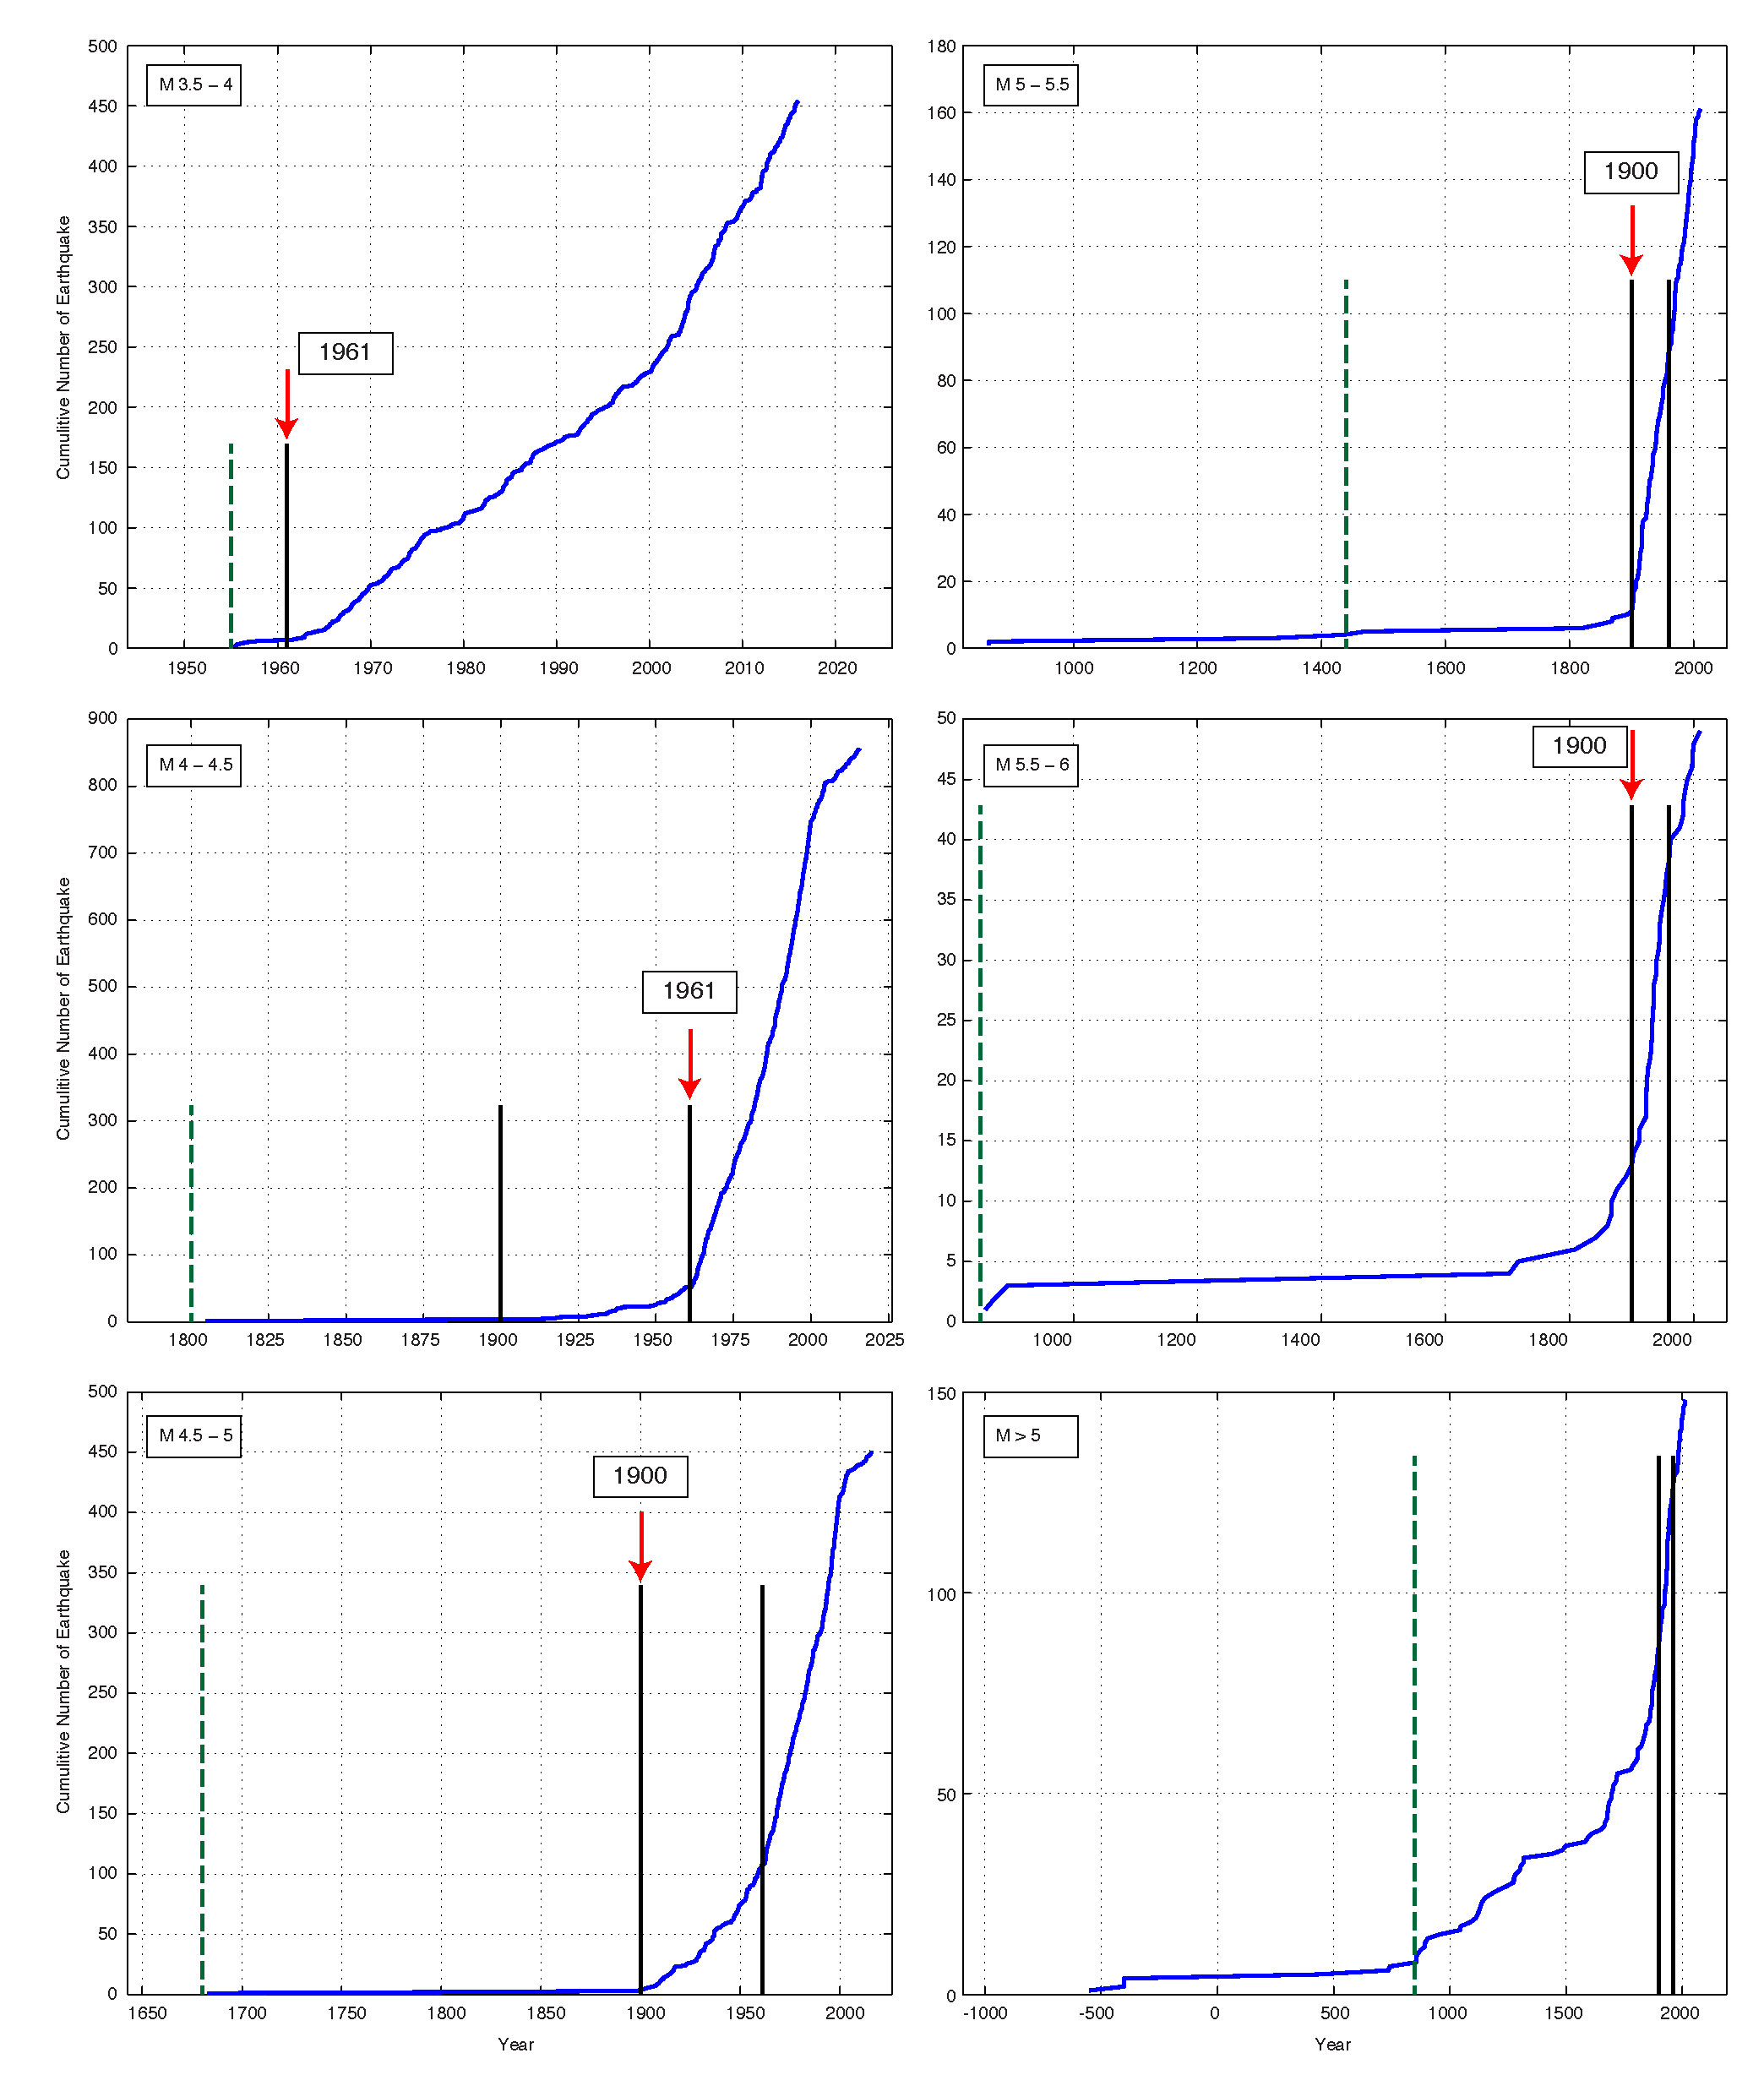
\includegraphics[scale=0.4]{figures/pdf/completness_compare_zare_2014_Az_Al.pdf} 
\caption{Cumulative number of earthquakes with respect to the time. Magnitude range is represented in a box at the top left corner. Solid black lines represent the starting of early instrumental (1900) and instrumental (1961) period. Green dashed lines represents the completeness threshold reported by \citet{Zare2014}. Arrows show the possible places to choose as completeness threshold after \citet{Frankel1995}.}
\label{fig:completness_compare_zare_2014_Az_Al}
\end{figure*}

\noindent
Fig.~\ref{fig:comp_test_all_mag} illustrates the completeness of data for each magnitude threshold in five different regions. A uniform rise of cumulative number of earthquake in each magnitude range, defines the threshold for catalog completeness. We define the completeness of each magnitude range at a time which the cumulative number of earthquake increase linearly with time. We assume the catalog for earthquakes with magnitude greater than  7 ($M_w > 7$) is complete from the first historical earthquake report.  Determining the completeness of the catalog for $ 6 < Mw \leq 7 $ needs precise observation of the catalog. In Azerbaijan tectonic seismic region after 1045  $Mw = 6.2$ earthquake the catalog seems complete up to 1318. However, between 1318 and 1581 (263 years) only one earthquake with magnitude $Mw > 6$ is reported (1440,  $Mw = 6.2$ ). Considering the activity of the Azerbaijan region, in this study we assume that the catalog is complete for earthquake with magnitude $ 6 < Mw \leq 7 $ after 1581. Similar situation happened at the period of 1715 - 1833. It worth to mention that in this case, the time period is shorter than before (118 years), meanwhile in this period of time two earthquakes with magnitude $Mw>7$ occurred in the Azerbaijan region (1721 $Mw=7.7$, 1780 $Mw=7.6$). The catalog may or may not be completed after 1045, however in this study we consider 1581 as a completeness threshold for magnitude  $ 6 < Mw \leq 7 $. Considering completeness of the catalog for Azerbaijan region from 1581 will result in conservative PGA for the region in comparison with the model with threshold of 1045. We picked the completeness threshold for other regions and other magnitude ranges according as a year that the cumulative number of earthquakes increment uniformly. Table ~\ref{tab:completeness} shows the summary of values used in this study.


\begin{figure*} [!ht]
\centering
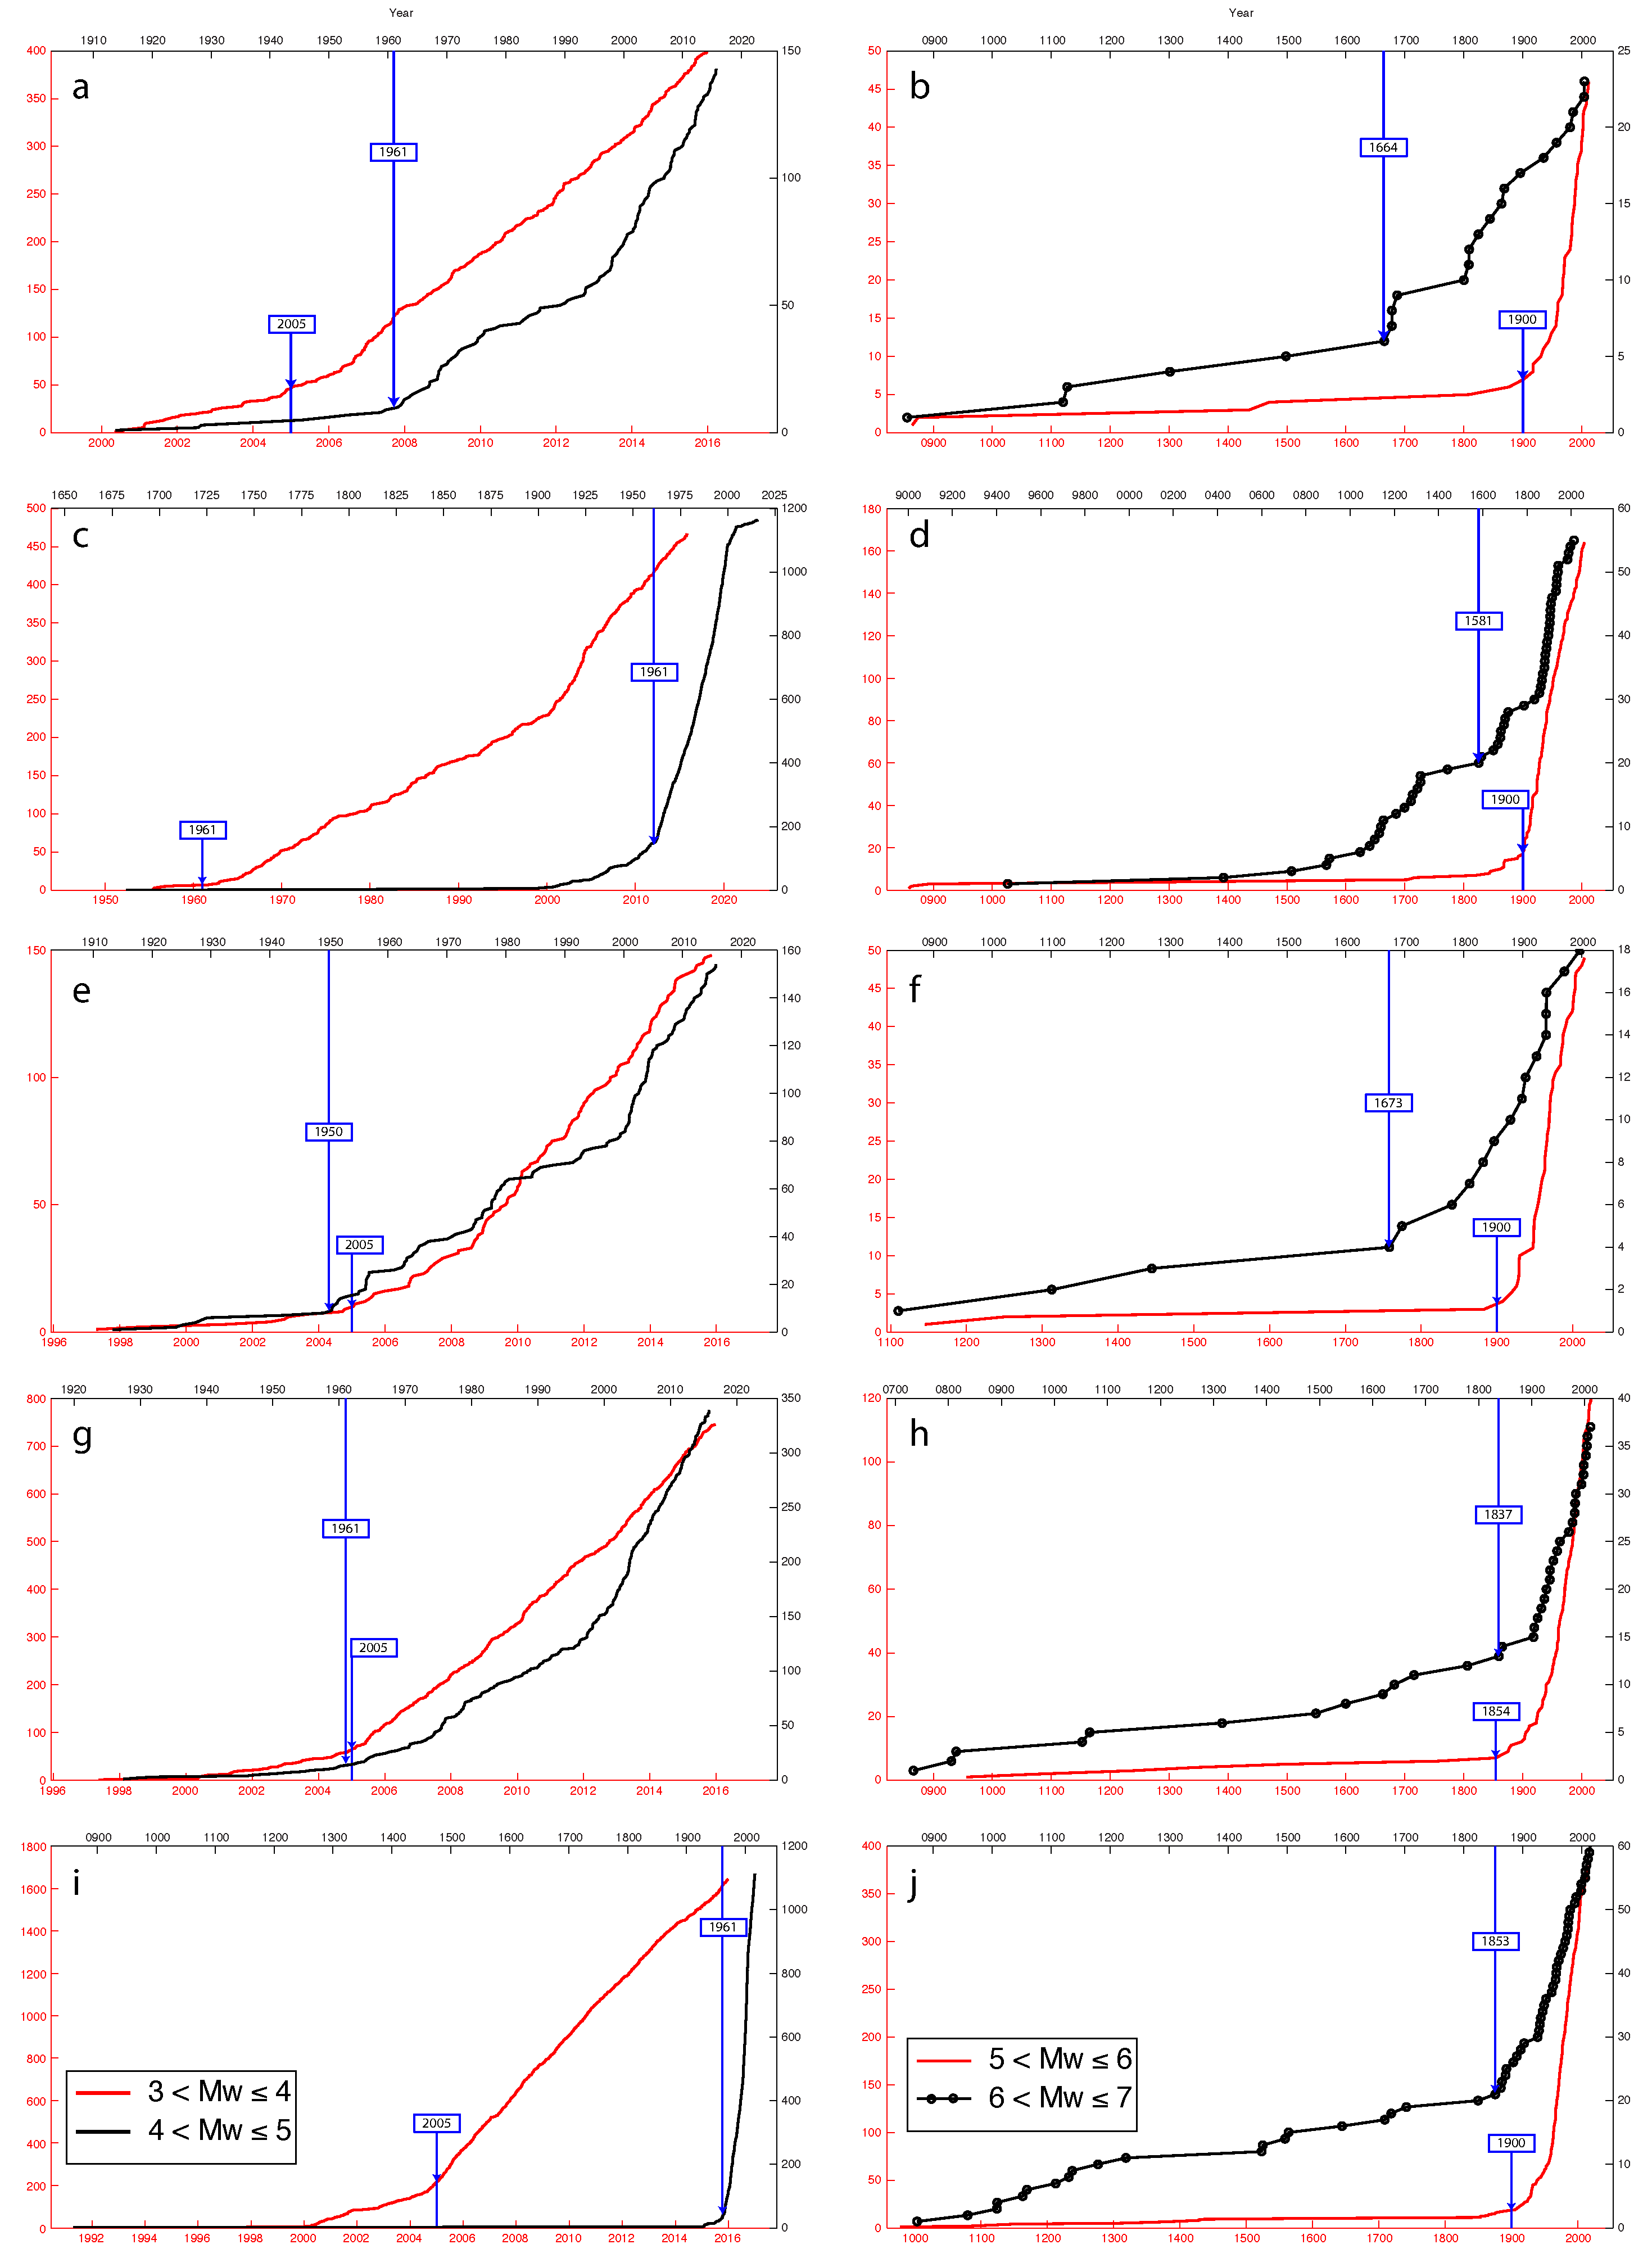
\includegraphics[scale=0.28]{figures/pdf/comp_test_all_mag.pdf} 
\caption{Magnitude-time distribution of earthquakes in the study regions. a-b) Alborz, c-d) Azerbaijan, e-f)Kopek Dagh, g-h)Kopeh Dagh, i-j)Zagros}
\label{fig:comp_test_all_mag}
\end{figure*}



\begin{table*}[!ht]
\centering
\caption{Completeness threshold of tectonic seismic regions.}
\begin{tabular}{ccccccccc}
 ~           & Azerbaijan & Alborz & Kopeh Dagh & Central Iran & Zagros & North Iran  \\ \hline
3-4         & 1961          & 2005   & 2005             & 2005            & 2005    & 2005          \\ \hline
4-5         & 1961          & 1961   & 1950             & 1961            & 1961    & 1961          \\ \hline
5-6         & 1900          & 1900   & 1900             & 1854            & 1900    & 1900           \\ \hline
6-7         & 1581          & 1664   & 1673             & 1837            & 1853    & 1778           \\ \hline
7 $< $    & 1042          & -401    & 9                   & 762              & 1439    & -401            \\ 
\end{tabular}
\label{tab:completeness}
\end{table*}














%% ---------------------------------------------
%% ---------------------------------------------
%
%% My (Naeem) original text.
%
%
%\section{Analysis Parameters}
%%\subsection{Magnitude Interval}
%%\subsection{Minimum Magnitude}
%\subsection{Attenuation Relationship}
%The choice of a ground motion attenuation model is of great importance since attenuation has proven to be a highly influential factor of seismic hazard. \citet{Zafarani2014} used 163 free-field acceleration time histories recorded at epicentral distance of up to 200 km from 32 earthquakes to investigate the predictive capabilities of the local, regional, and next generation attenuation (NGA) ground-motion prediction equations and determined their applicability for northern Iran. After evaluating different Ground Motion Prediction Equations, \citet{Kalkan2004}, \citet{Chiou2008}, and \citet{Boore2008} represented suitable performance for  PGA  with LLH (Log-Likelihood method) score of 1.54, 1.55, and 1.59. Mean of the mentioned attenuation relationships (not shown here), are very close together, especially at higher magnitude. Using \citet{Scherbaum2009} approach and \citet{Zafarani2014} coefficients we calculated the logic tree weights as 0.3376, 0.3354, and 0.3270, respectively. Getting close mean values and logic tree weights, in order to consider the epistemic uncertainty, instead of using several GMPEs we use the top rank GMPE (i.e.  \citet{Kalkan2004} ). We also presented the results for  $\pm$ standard deviation. \\
%
%\noindent
%The attenuation relationship is:
%
%\begin{equation}
%\begin{split}
%ln\ (Y) = b_1 + b_2(M_w-6) + b_3( M_w-6)^{2}+  \\ 
%b_5ln\ r + b_V \ ln(V_S/V_A) \  with \  r= \sqrt{R{r^2_{cl} + h^2}}  
%\end{split}
%\end{equation}
%
%where $Y$ is in $g$, $b_1 = 0.393$, $b_2 = 0.576$, $b_3 = -0.107$, $b_5 = -0.899$, $b_V = -0.200$, $V_A = 1112$, $h(km) = 6.91$, $\sigma_{ln\ Y} = 0.612$.
%
%\subsection{b-value}
%
%For each of the three seismic regions, Gutenberg-Richter parameters and Max magnitude ($M_{max}$) were calculated using Seismic Hazard Assessment code (HA3) \citep{kijko2004}. The regional maximum magnitude for each region is estimated by the \citet{Kijko1989} method, which is implemented in the HA3 package. For smoothed seismicity areas, $b-value$ is assumed constant. The $a-value$ can vary spatially and is determined by counting earthquakes above $M$ 3.0 in each grid cells.\\
%\noindent
%\citet{Karimiparidari2013} applied the Maximum Curvature (MAXC) technique \citep{Wyss1999, Wiemer2000} by ZMap \citep{Wiemer2001} to calculate the level of completeness of instrumental part of the catalog.  Following the \citet{Karimiparidari2013}, we assume the catalog is complete for earthquakes with magnitude 4.5, 4.4, 4.5, 4.5, and 4.4 for Azerbaijan, Alborz,  Kopeh-Dagh, Central Iran, and Zagros tectonic seismic regions, respectively. For the north Iran uniform model we used 4.5 as a completeness magnitude. In this study we use those magnitudes of completeness as the magnitude threshold in the calculation of the seismicity parameters. We also used the seismicity parameters of this study \citep{Karimiparidari2013} as the priory information in HA3 code. The updated values are displayed in Table \ref{tab:b_value}.  Annual occurrence rate of the earthquake for each region is shown in Fig.~\ref{fig:annual_m}.
%
%\begin{figure*} [!ht]
%\centering
%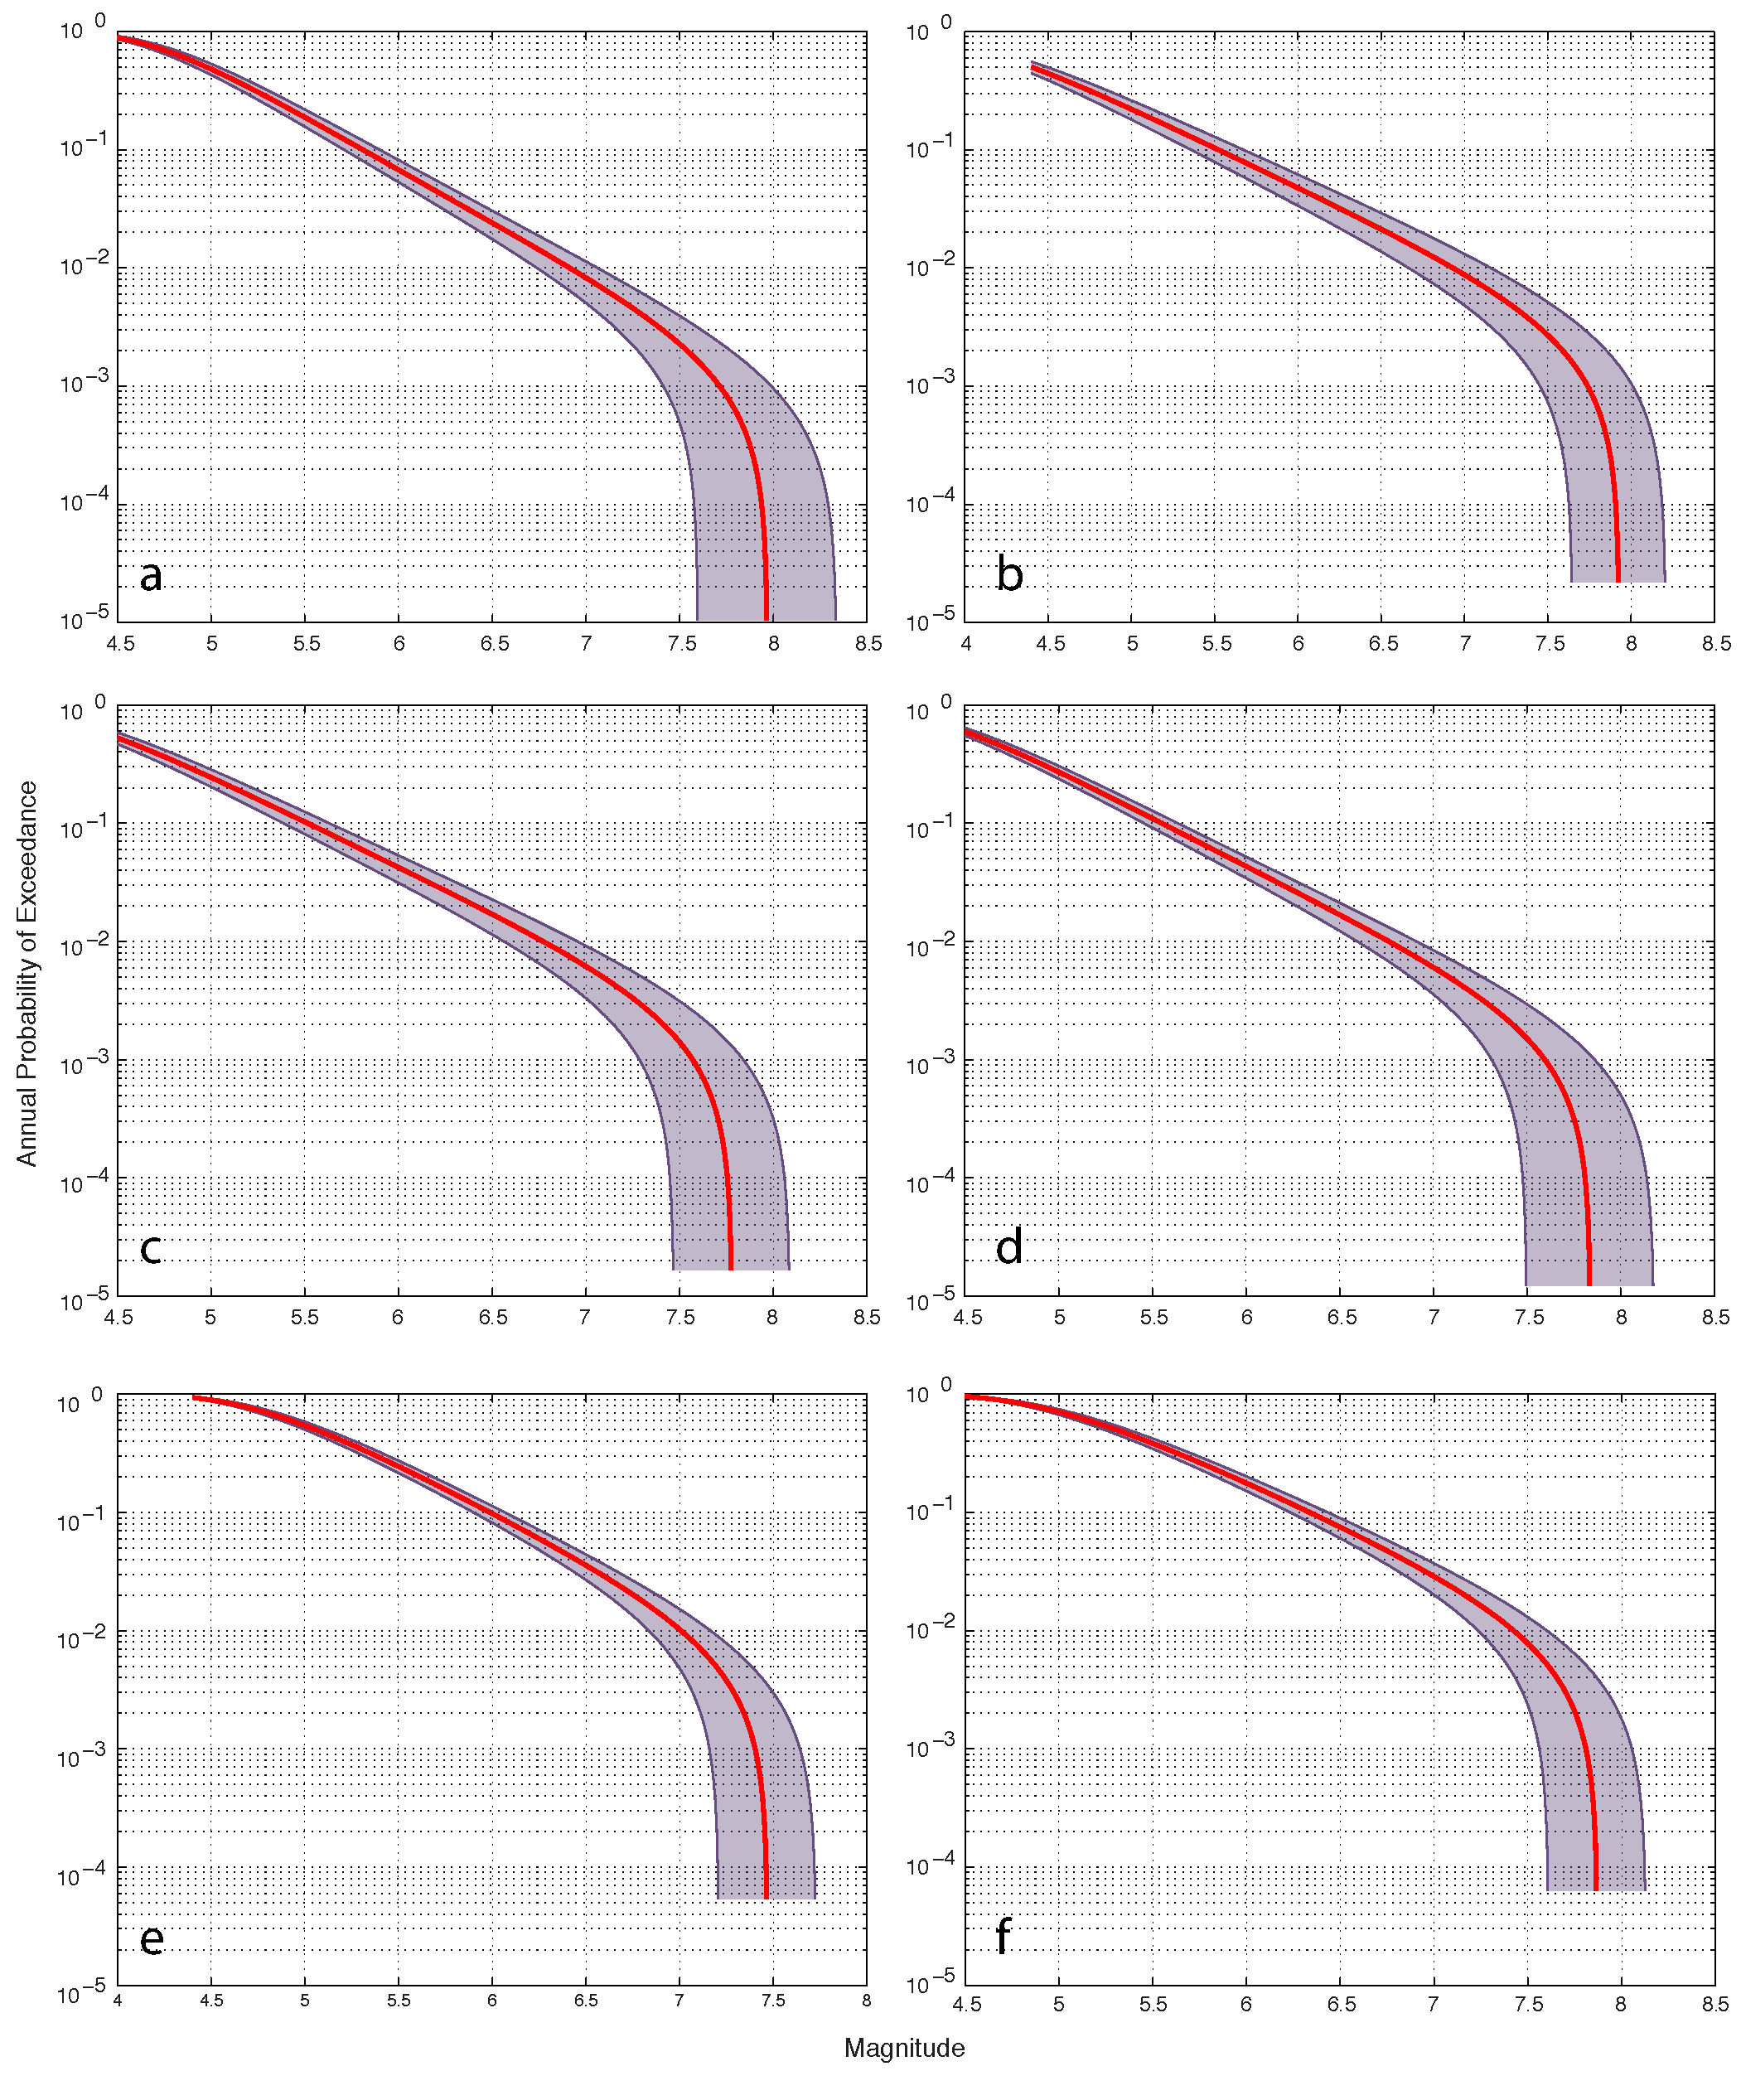
\includegraphics[scale=0.4]{figures/pdf/annual_rate_m.pdf} 
%\caption{Annual occurrence rate of the earthquake. a) Azerbaijan, b) Alborz, c) KopehDagh, d)Central, e)Zagros f) North Iran}
%\label{fig:annual_m}
%\end{figure*}
%
%
%
%
%\noindent
%
%
%\begin{table*}[!ht]
%\centering
%\caption{Seismicity parameters for three tectonic seismic regions.}
%    \begin{tabular}{ccccc}
%    ~                          &         $b-value$     &   $M_{max} $  Calculated & $M_{max}$ obseved \\ \hline
%    Azerbaijan           & 1.1   $\pm$ 0.03   &   7.93  $\pm$  0.34           &   7.7      			    \\ \hline
%    Alborz                  &1.03  $\pm$ 0.03   &   7.85  $\pm$  0.66           &   7.8          	            \\ \hline
%    Kopeh Dagh        & 0.89 $\pm$ 0.04   &   7.78  $\pm$  0.31           &   7.6          	            \\ \hline
%    Central Iran         & 0.95 $\pm$ 0.04   &   7.84  $\pm$  0.34           &   7.6                           \\ \hline
%    Zagros                 & 0.99 $\pm$ 0.02  &   7.47  $\pm$  0.26            &  7.4                            \\ \hline
%    Uniform Model    & 0.9    $\pm$ 0.02  &   7.87  $\pm$  0.26            &  7.8                            \\ 
%    \end{tabular}
% \label{tab:b_value} 
%\end{table*}
%
%
%\subsection{Catalog Completness}
%For the smoothed seismicity method, completeness of each magnitude in the catalog is an important factor.  \citet{Frankel1995} plotted the cumulative number of events against time for different regions. He assumes that from the point that the line become linear, the catalog is complete. Using the cumulative frequency-magnitude distribution of \citet{Gutenberg1944} and also frequency magnitude distribution approach in software ZMAP \citep{Wiemer2001}, \citet{Zare2014} reported the catalog completeness for the study regions. World widely large earthquakes were routinely located after increasing number of seismic stations establishment in the early 1900s \citep{Shearer2009}. Up to 1961 these data formed the early instrumental period. In 1961 the Worldwide Standardized Seismograph Network (WWSSN) was stablished. The record of these seismographs considerably improved the seismic catalogs in different part of the world \citep{Shearer2009}. Fig.~\ref{fig:completness_scatter} shows the magnitude distribution of events with respect to the time of occurrence of the events.
%
%\begin{figure*} [!ht]
%\centering
%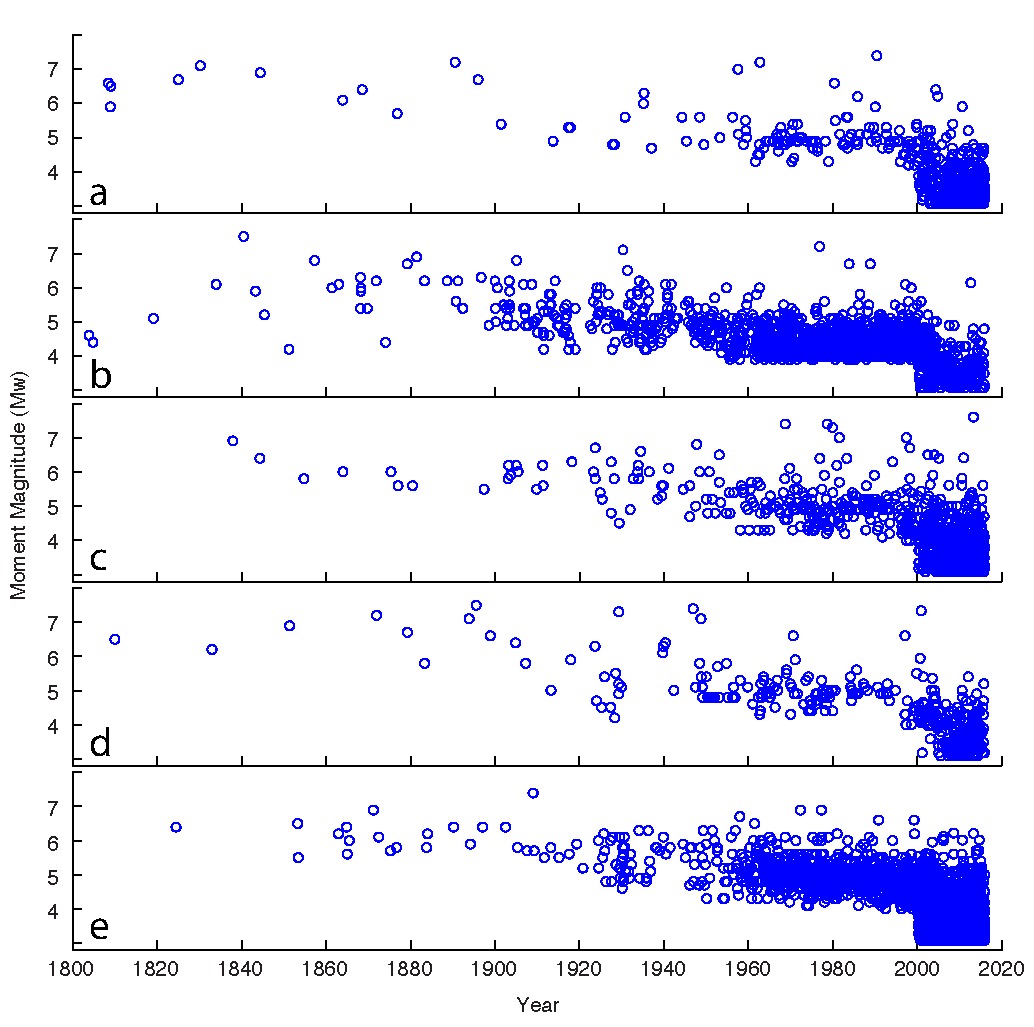
\includegraphics[scale=0.6]{figures/pdf/completness_scatter.pdf} 
%\caption{Magnitude-time distribution of earthquakes in the study regions. a) Alborz, b) Azerbaijan, c)Central, d)Kopeh-Dagh, e)Zagros}
%\label{fig:completness_scatter}
%\end{figure*}
%
% According to   \citet{Frankel1995},  we made plots of the cumulative number of events against time for different regions' catalog. We pick the Mw 0.5 increments in magnitude to be able to compare the results with \citet{Zare2014}. In order to be able to compare the results with \citet{Zare2014} we merge the data of Azerbaijan and Alborz seismic regions.  Fig.~\ref{fig:completness_compare_zare_2014_Az_Al} shows the completeness of catalog for earthquakes with different magnitude range in Azerbaijan-Alborz region. According to this figure, midrange magnitudes ($ 4 < Mw < 6 $) fairly obey the network developments in 1900 and 1961. The completeness thresholds for each magnitude range which are reported by \citet{Zare2014} are shown by dashed green line. In this study we follow the \citet{Frankel1995} approach to determine the completeness of each region. Even though the approach used by \citet{Frankel1995} will lead to the conservative results, we make sure that we don't use a period of time without knowing the complete number of events. Determining the completeness of the catalog is very sensitive to the data. Converting earthquake magnitudes from different scales to moment magnitude obviously has some error. Having broader range of magnitude will help to minimize these sort of error. In this study we consider the magnitude intervals for completeness study as $Mw = 1$. 
%
%\begin{figure*} [!ht]
%\centering
%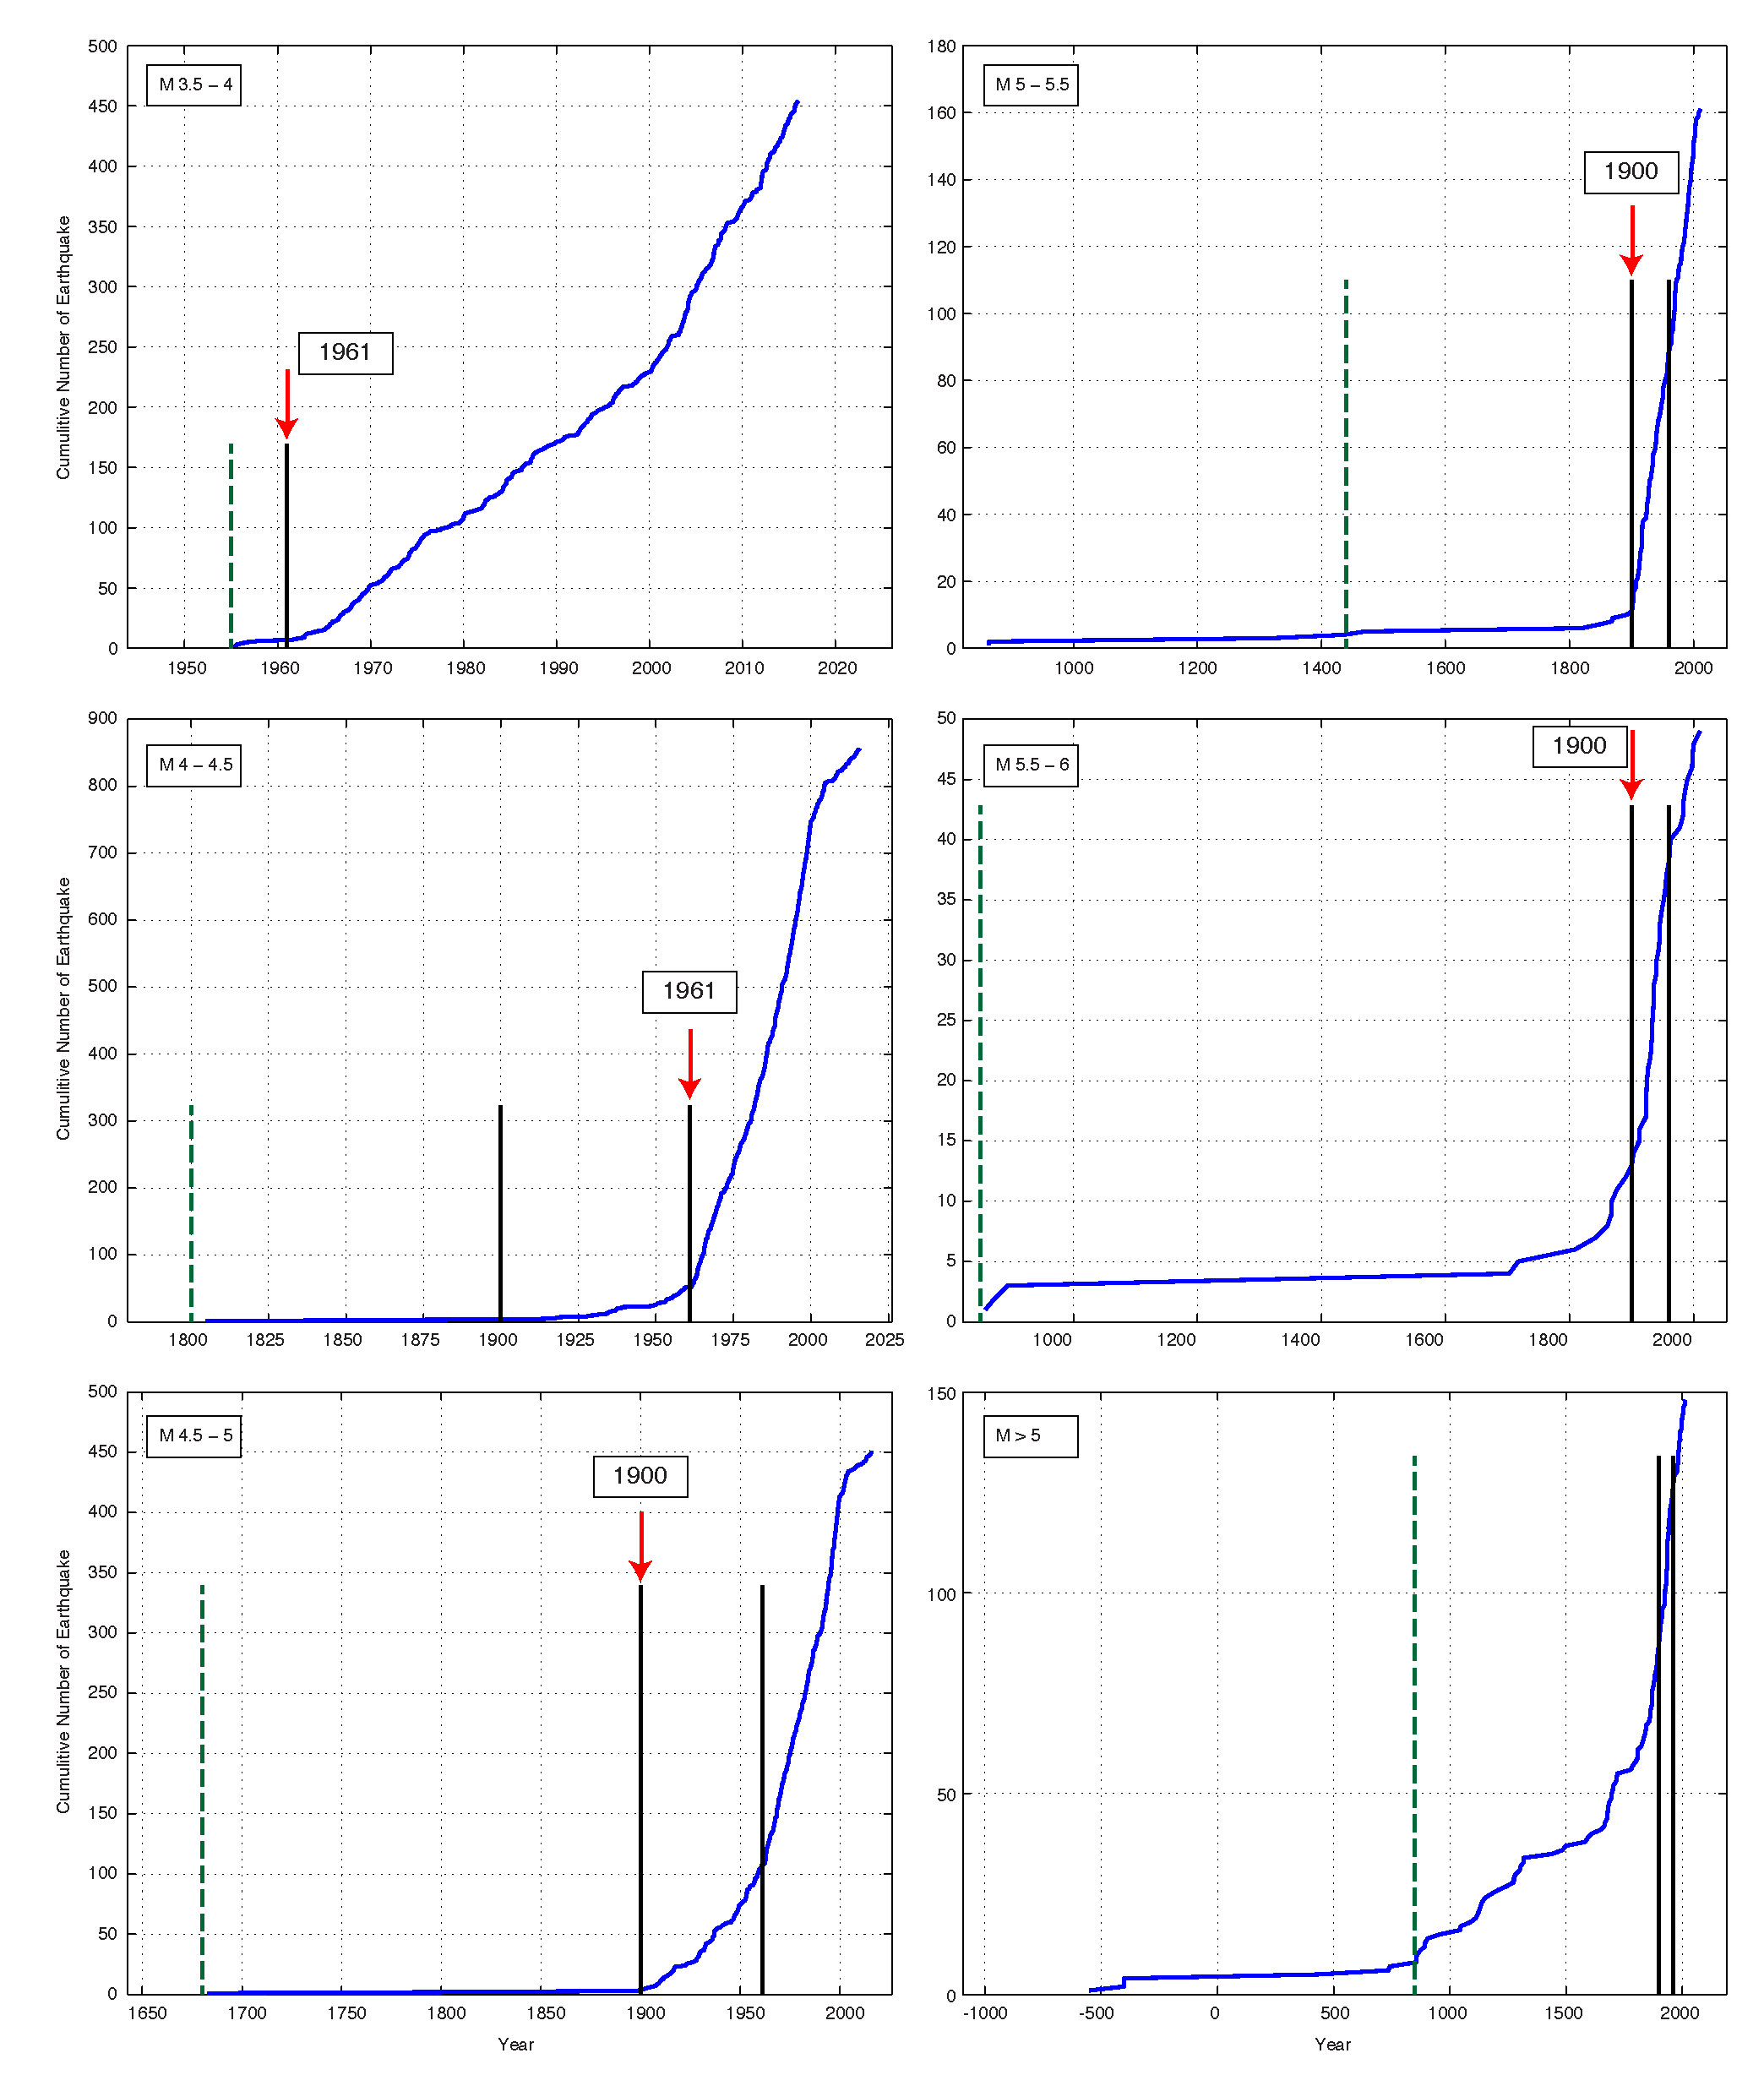
\includegraphics[scale=0.4]{figures/pdf/completness_compare_zare_2014_Az_Al.pdf} 
%\caption{Cumulative number of earthquakes with respect to the time. Magnitude range is represented in a box at the top left corner. Solid black lines represent the starting of early instrumental (1900) and instrumental (1961) period. Green dashed lines represents the completeness threshold reported by \citet{Zare2014}. Arrows show the possible places to choose as completeness threshold after \citet{Frankel1995}.}
%\label{fig:completness_compare_zare_2014_Az_Al}
%\end{figure*}
%
%\noindent
%Fig.~\ref{fig:comp_test_all_mag} illustrates the completeness of data for each magnitude threshold in five different regions. A uniform rise of cumulative number of earthquake in each magnitude range, defines the threshold for catalog completeness. We define the completeness of each magnitude range at a time which the cumulative number of earthquake increase linearly with time. We assume the catalog for earthquakes with magnitude greater than  7 ($M_w > 7$) is complete from the first historical earthquake report.  Determining the completeness of the catalog for $ 6 < Mw \leq 7 $ needs precise observation of the catalog. In Azerbaijan tectonic seismic region after 1045  $Mw = 6.2$ earthquake the catalog seems complete up to 1318. However, between 1318 and 1581 (263 years) only one earthquake with magnitude $Mw > 6$ is reported (1440,  $Mw = 6.2$ ). Considering the activity of the Azerbaijan region, in this study we assume that the catalog is complete for earthquake with magnitude $ 6 < Mw \leq 7 $ after 1581. Similar situation happened at the period of 1715 - 1833. It worth to mention that in this case, the time period is shorter than before (118 years), meanwhile in this period of time two earthquakes with magnitude $Mw>7$ occurred in the Azerbaijan region (1721 $Mw=7.7$, 1780 $Mw=7.6$). The catalog may or may not be completed after 1045, however in this study we consider 1581 as a completeness threshold for magnitude  $ 6 < Mw \leq 7 $. Considering completeness of the catalog for Azerbaijan region from 1581 will result in conservative PGA for the region in compare with the model with threshold of 1045. We picked the completeness threshold for other regions and other magnitude ranges according as a year that the cumulative number of earthquakes increment uniformly. Table ~\ref{tab:completeness} shows the summary of values used in this study.
%
%
%
%\begin{figure*} [!ht]
%\centering
%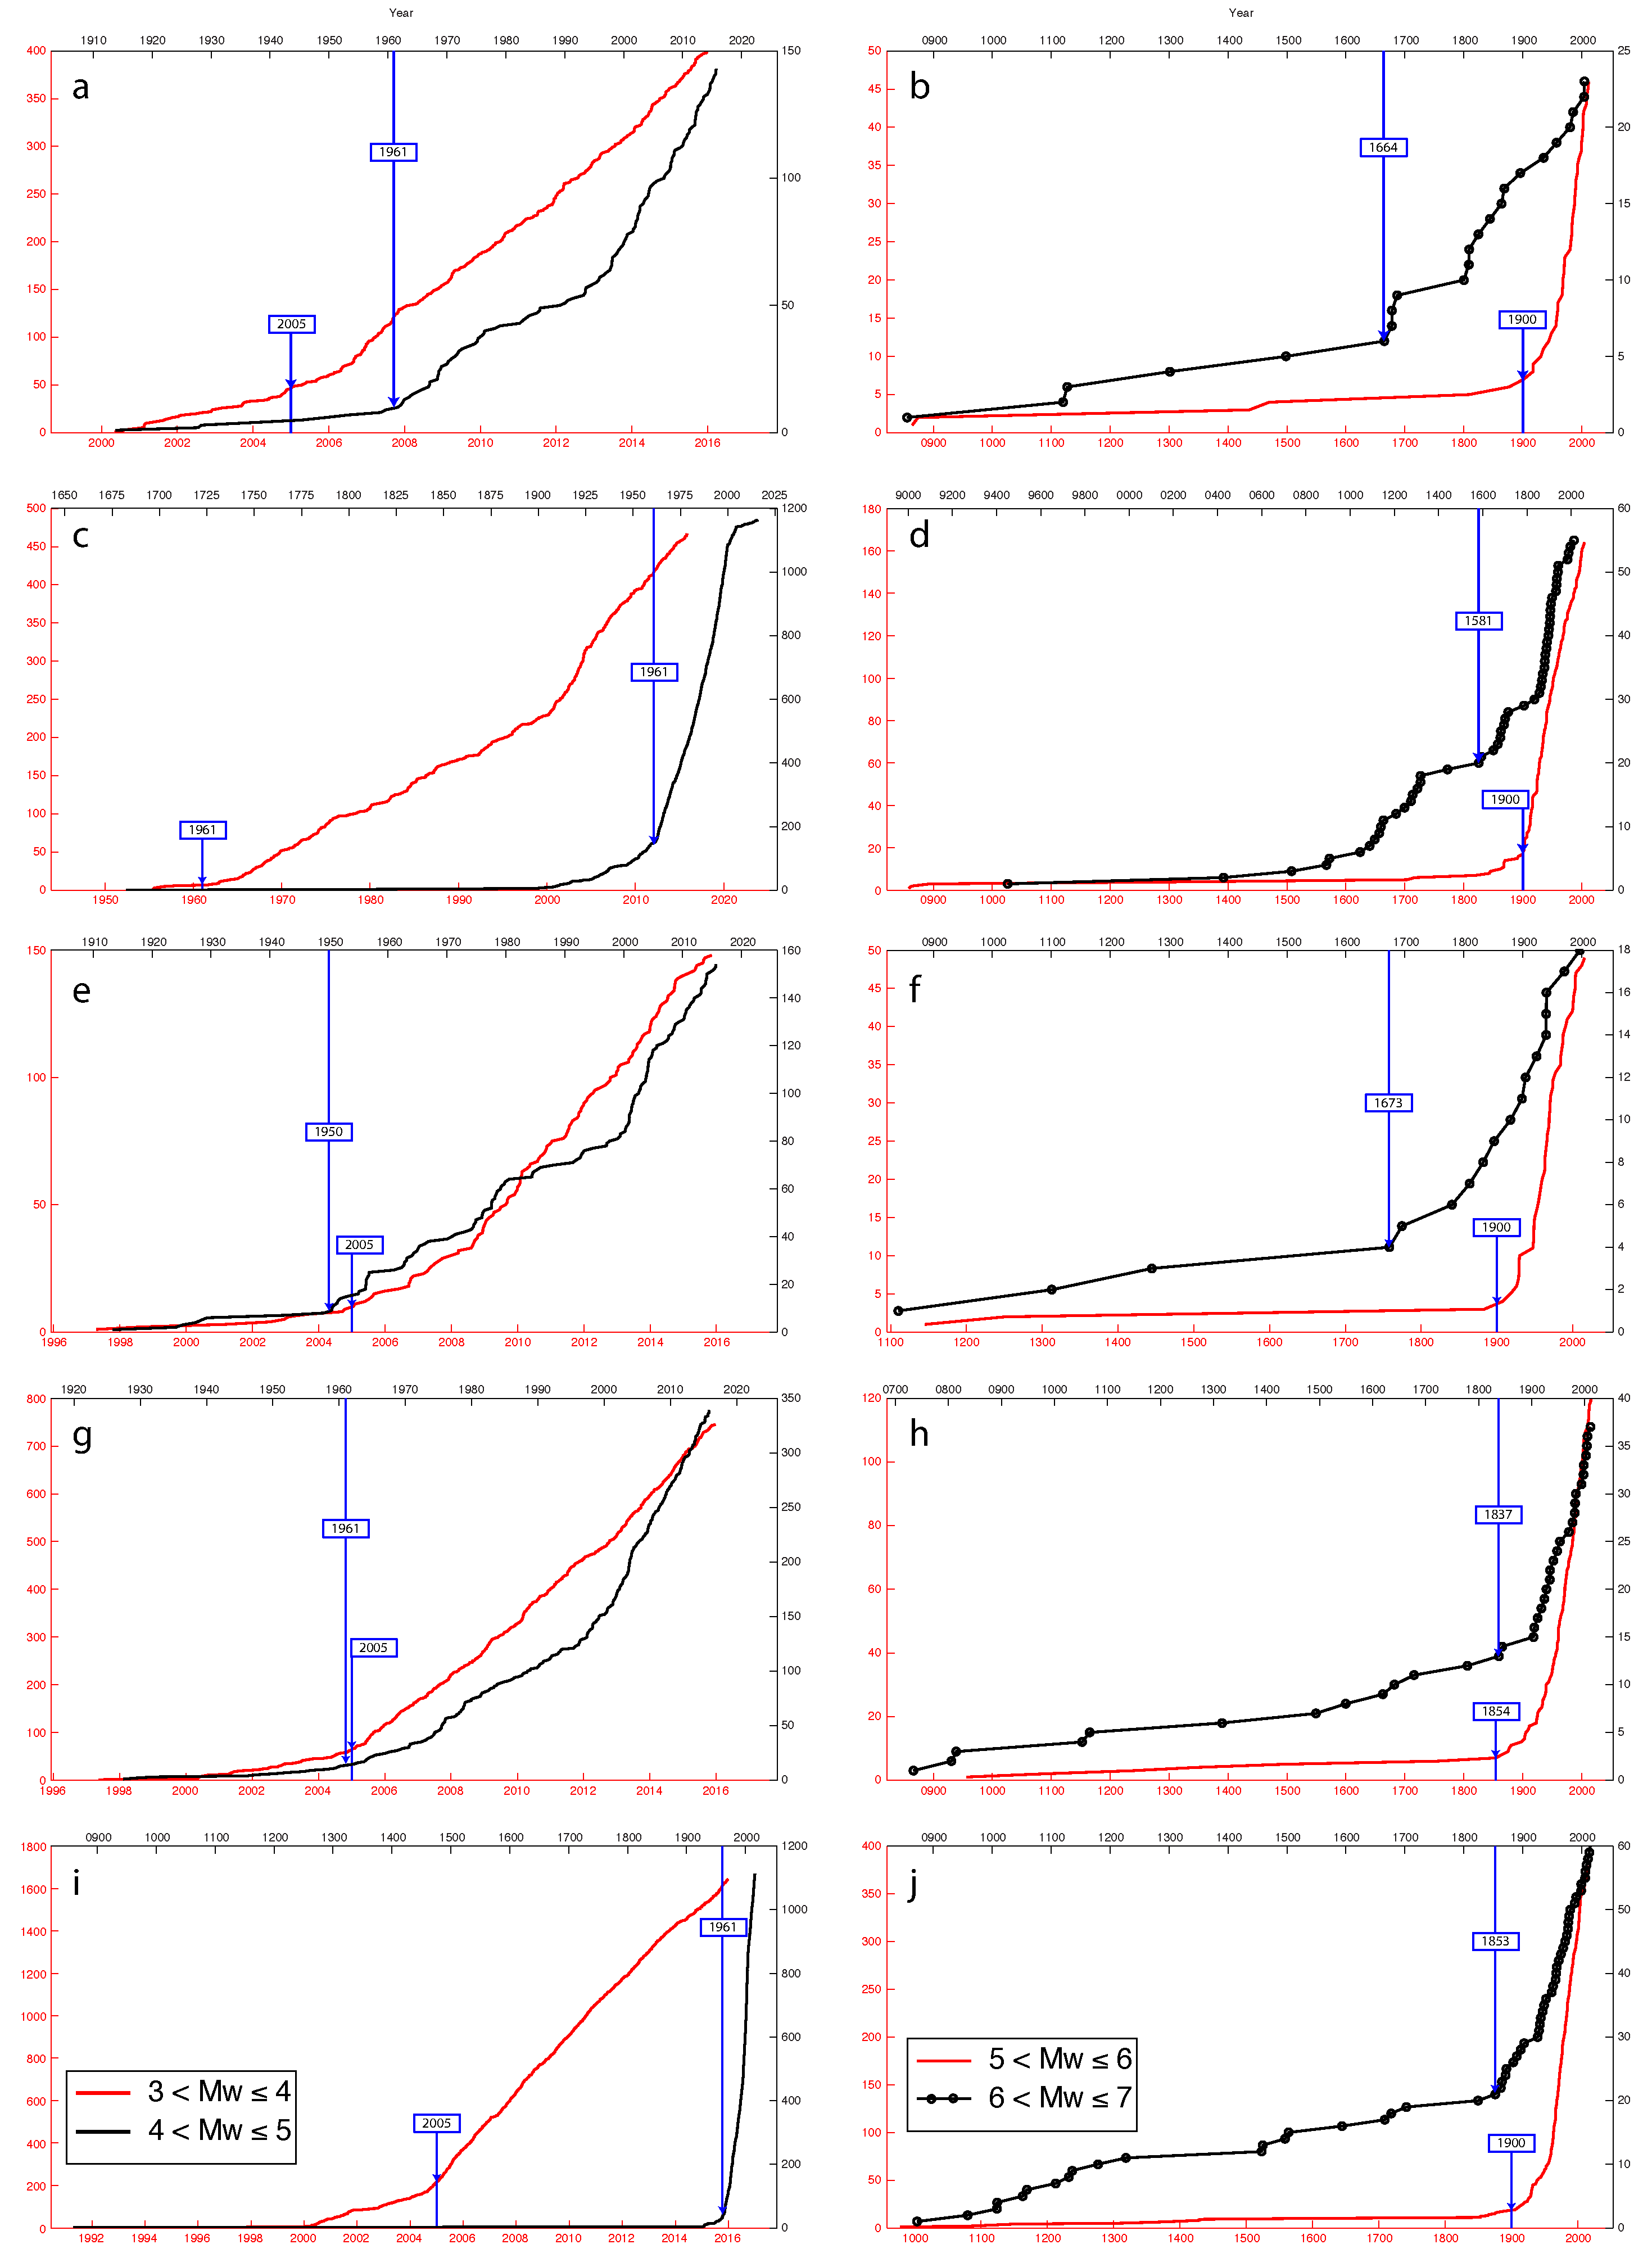
\includegraphics[scale=0.28]{figures/pdf/comp_test_all_mag.pdf} 
%\caption{Magnitude-time distribution of earthquakes in the study regions. a-b) Alborz, c-d) Azerbaijan, e-f)Kopek Dagh, g-h)Kopeh Dagh, i-j)Zagros}
%\label{fig:comp_test_all_mag}
%\end{figure*}
%
%
%
%\begin{table*}[!ht]
%\centering
%\caption{Completeness threshold of tectonic seismic regions.}
%\begin{tabular}{ccccccccc}
% ~           & Azerbaijan & Alborz & Kopeh Dagh & Central Iran & Zagros & North Iran  \\ \hline
%3-4         & 1961          & 2005   & 2005             & 2005            & 2005    & 2005          \\ \hline
%4-5         & 1961          & 1961   & 1950             & 1961            & 1961    & 1961          \\ \hline
%5-6         & 1900          & 1900   & 1900             & 1854            & 1900    & 1900           \\ \hline
%6-7         & 1581          & 1664   & 1673             & 1837            & 1853    & 1778           \\ \hline
%7 $< $    & 1042          & -401    & 9                   & 762              & 1439    & -401            \\ 
%\end{tabular}
%\label{tab:completeness}
%\end{table*}
